\documentclass[11pt]{article}

\usepackage[margin=1in]{geometry}
\usepackage{amsmath, amssymb}
\usepackage{listings}
\usepackage{xcolor}
\usepackage{hyperref}
\usepackage{enumitem}
\usepackage{titlesec}
\usepackage{parskip}
\usepackage{booktabs}
\usepackage{tcolorbox}
\usepackage{tikz}
\usetikzlibrary{arrows.meta, positioning, shapes.geometric}

\lstset{
    basicstyle=\ttfamily\small,
    keywordstyle=\color{blue}\bfseries,
    commentstyle=\color{gray}\itshape,
    stringstyle=\color{red},
    frame=single,
    breaklines=true,
    showstringspaces=false,
    tabsize=4
}

\newtcolorbox{keyidea}[1][]{colback=blue!5, colframe=blue!50!black,
    fonttitle=\bfseries, title=Key Idea, #1}

\newtcolorbox{keytip}[1][]{colback=green!5, colframe=green!50!black,
    fonttitle=\bfseries, title=Tip, #1}

\newtcolorbox{keyintuition}[1][]{colback=orange!5, colframe=orange!50!black,
    fonttitle=\bfseries, title=Intuition, #1}

\title{\textbf{CS3210: Operating Systems} \\ Lecture 8 --- Virtual Memory: Copy-on-Write}
\author{John Kim \\ Georgia Institute of Technology}
\date{February 10, 2026}

\begin{document}
\maketitle
\tableofcontents
\newpage

% ============================================================
\section{Review: Software Page Walk with \texttt{walkpgdir}}
% ============================================================

The heart of xv6's virtual memory system is the \textbf{software page walk}, implemented by the \texttt{walkpgdir} function in \texttt{vm.c}. This function translates a virtual address to a page table entry (PTE), which can then be inspected or modified. Understanding this function is essential before tackling Copy-on-Write, because CoW implementation hinges on being able to intercept and manipulate PTEs.

The \textbf{page walk} works as follows: given a page directory (the top-level page table), a virtual address, and an allocation flag, \texttt{walkpgdir} returns a pointer to the PTE corresponding to that virtual address. If the page table does not exist and allocation is requested, it allocates a new page table. The function uses three key macros to extract parts of the virtual address:

\begin{itemize}
    \item \textbf{PDX(va)}: extracts bits [31:22], the page directory index (upper 10 bits).
    \item \textbf{PTX(va)}: extracts bits [21:12], the page table index (middle 10 bits).
    \item \textbf{PTE\_ADDR(pte)}: masks off the lower 12 flag bits, leaving the 20-bit physical page number.
\end{itemize}

Here is the \texttt{walkpgdir} implementation:

\begin{lstlisting}[language=C, caption={The \texttt{walkpgdir} function from xv6 vm.c}]
static pte_t *walkpgdir(pde_t *pgdir, const void *va, int alloc) {
    pde_t *pde;
    pte_t *pgtab;

    pde = &pgdir[PDX(va)];
    if(*pde & PTE_P) {
        pgtab = (pte_t*)P2V(PTE_ADDR(*pde));
    } else {
        if(!alloc || (pgtab = (pte_t*)kalloc()) == 0)
            return 0;
        memset(pgtab, 0, PGSIZE);
        *pde = V2P(pgtab) | PTE_P | PTE_W | PTE_U;
    }
    return &pgtab[PTX(va)];
}
\end{lstlisting}

The function's logic is straightforward. First, it computes a pointer to the page directory entry (PDE) corresponding to the upper 10 bits of the virtual address. If the PDE indicates a present page table (PTE\_P flag set), the function fetches the physical address stored in the PDE, converts it to a kernel virtual address using \texttt{P2V}, and treats it as a page table. If the page table is not present and allocation is requested, \texttt{walkpgdir} allocates a fresh 4~KB page via \texttt{kalloc}, initializes it to zero, and installs a PDE pointing to it with the P (Present), W (Writable), and U (User) flags set. Finally, it indexes into the page table using the middle 10 bits of the virtual address and returns the address of the corresponding PTE.

This function is the workhorse of virtual memory manipulation in xv6. Page protection changes, TLB flushing decisions, and CoW bookkeeping all flow through or depend on understanding the PTEs discovered by \texttt{walkpgdir}.

% ============================================================
\section{xv6 VMM Limitations and Opportunities}
% ============================================================

The xv6 virtual memory system, while functional, has fundamental design decisions that differ sharply from production operating systems. Understanding these limitations reveals why Copy-on-Write is not only useful but nearly impossible to implement correctly in xv6's current architecture, and it motivates the opportunities that CoW unlocks in other systems.

\textbf{Current xv6 design:} xv6 maintains a simple one-to-one mapping between logical physical pages and usage. At most, one kernel page table and one user page table can map to any given physical page. There is no support for \emph{many-to-one mappings}, where multiple virtual pages (possibly from different page tables or different processes) map to a single physical frame. This design choice, while simple, forecloses several important OS features.

\textbf{Physical memory management:} xv6 requires the kernel to maintain a virtual mapping for all physical memory up to 2~GB. This is done in \texttt{setupkvm} and used throughout the kernel to manipulate memory directly. Any user program can request free physical pages and map them into its virtual address space via \texttt{kalloc} and page table setup. Once the kernel and one user process have mappings to a physical page, the page is marked as in-use and no other process can claim it. The physical page tracking is binary: free or allocated. There is no reference counting or multiple ownership.

\textbf{Limitations and consequences:} Because xv6 forbids many-to-one mappings, implementing Copy-on-Write fork is nearly impossible. In a CoW fork, the parent and child processes must share the same physical pages (many-to-one), with those pages marked read-only. When either process attempts to write, the OS traps the fault, allocates a new frame, copies the shared page into it, and updates the faulting process's page table. But xv6's page reference counting is primitive, and there is no mechanism to track how many processes hold a mapping to a given physical page. Equally, shared library mapping—where a single copy of a library's code and read-only data occupies one physical page mapped by multiple processes—becomes cumbersome without proper many-to-one support.

\textbf{Opportunities in other systems:} Production operating systems like Linux, Windows, and macOS all support many-to-one mappings and reference-count physical pages. This enables Copy-on-Write fork (reducing fork latency from $O(n)$ to $O(1)$ amortized), shared memory regions, memory-mapped files with precise lazy copying, and deduplication. The OS must track, for each physical page, how many processes hold a mapping to it. This reference count determines when a page can be freed and when a CoW page must be duplicated on write.

% ============================================================
\section{Virtual Memory Tips and Tricks: Interpose and Suspend Reality}
% ============================================================

Paging is one of the most powerful tools in the OS designer's arsenal because it is a \textbf{level of indirection} between the process's view of memory and the physical reality. This indirection allows the OS to observe, intercept, and modify memory behavior transparently.

Consider what the OS can do once paging is in place. The OS observes memory accesses indirectly through the Accessed (A) and Dirty (D) bits set automatically by the MMU whenever a page is read or written. By consulting these bits, the OS learns the access pattern of a process without instrumenting every memory operation. The OS can change page table entries on the fly, remapping virtual pages to different physical frames or changing protection bits, without the process knowing. This is the mechanism behind virtual memory management, swapping, and memory-mapped I/O.

The OS can also \textbf{interpose on the control path} by triggering page faults. A page fault is a synchronous exception that hands control to the OS, allowing the OS to inspect the faulting address, the faulting process, and the reason for the fault. The OS can then decide how to respond: allocate a page, bring in a swapped page, handle Copy-on-Write, or deny access. This is the closest the OS gets to a hook into every memory access without the overhead of software instrumentation.

\begin{keyintuition}
Paging lets the OS \textit{lie and be lazy}. The page table is the OS's ledger: it says ``this virtual page points to this physical page with these permissions.'' The OS can set permissions to be more restrictive than what is logically necessary, deferring real work until a fault occurs. This is suspension of reality: the process thinks it has full permission to write to a page, but the OS has marked it read-only to be informed when the first write occurs.
\end{keyintuition}

This concept is the seed of Copy-on-Write. The OS can fork a process, mark the child's pages read-only (even though they are logically writable), and defer the actual copying until the child (or parent) writes. The OS thereby trades a synchronous cost (copying all of memory) for asynchronous costs (handling write faults).

% ============================================================
\section{Copy-on-Write Fork: The Inefficient xv6 Status Quo}
% ============================================================

To appreciate Copy-on-Write, it helps to first understand what xv6 currently does when forking a process, and why it is inefficient.

In the current xv6 \texttt{fork} implementation, when a parent process calls \texttt{fork()}, the OS must fully copy the parent's entire virtual address space to the child. Let us consider a concrete example: a parent process with three mapped pages:

\begin{itemize}
    \item Virtual address 0x0000 $\rightarrow$ physical frame P1, containing 0xcafe.
    \item Virtual address 0x1000 $\rightarrow$ physical frame P2, containing 0xbeef.
    \item Virtual address 0x2000 $\rightarrow$ physical frame P3, containing 0x0507.
\end{itemize}

Upon fork, xv6 allocates three \emph{new} physical frames (P1', P2', P3') and copies the contents of P1, P2, and P3 into them. The child's page directory points to the child's page tables, which map the child's virtual addresses to the new physical frames. After the fork, six physical frames are in use: three belong to the parent, three to the child. The parent's memory is logically independent from the child's.

\begin{figure}[h]
\begin{center}
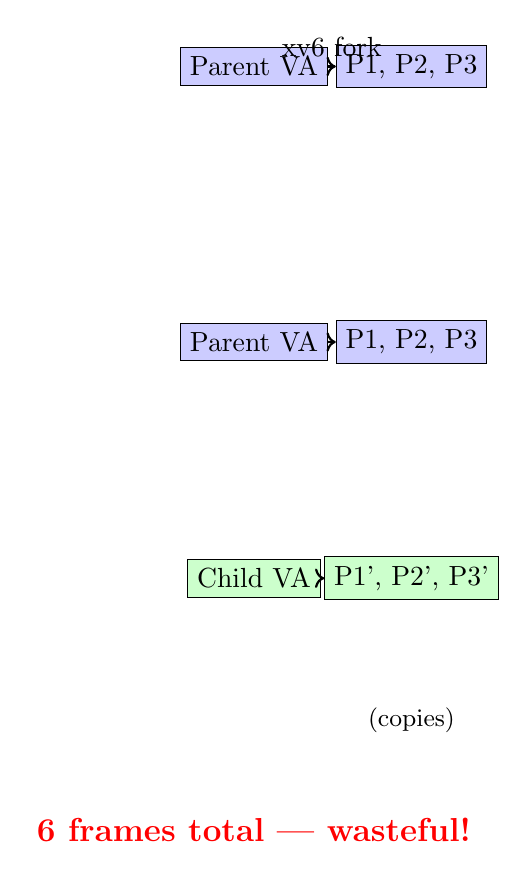
\begin{tikzpicture}[node distance=2cm, scale=0.85]
    % Parent side
    \node[rectangle, draw, fill=blue!20] (parent_addr) {Parent VA};
    \node[rectangle, draw, fill=blue!20, right of=parent_addr] (parent_frame) {P1, P2, P3};
    \draw[->, thick] (parent_addr) -- (parent_frame) node[midway, above] {xv6 fork};

    % After fork
    \node[rectangle, draw, fill=blue!20, below of=parent_addr, yshift=-1.5cm] (parent_addr_after) {Parent VA};
    \node[rectangle, draw, fill=blue!20, right of=parent_addr_after] (parent_frame_after) {P1, P2, P3};
    \draw[->, thick] (parent_addr_after) -- (parent_frame_after);

    \node[rectangle, draw, fill=green!20, below of=parent_addr_after, yshift=-1cm] (child_addr) {Child VA};
    \node[rectangle, draw, fill=green!20, right of=child_addr] (child_frame) {P1', P2', P3'};
    \node[below of=child_frame, yshift=0.2cm, font=\small] {(copies)};
    \draw[->, thick] (child_addr) -- (child_frame);

    % Inefficiency label
    \node[below of=child_addr, yshift=-1.2cm, font=\large\bfseries, color=red] {\textbf{6 frames total} --- wasteful!};
\end{tikzpicture}
\end{center}
\caption{xv6's current fork: full data copy. Parent and child each have their own physical pages, even though content is initially identical.}
\end{figure}

The cost of this approach is proportional to the address space size: if a process has $n$ pages, fork costs $O(n)$ in time (for copying) and space (keeping two full copies in memory). For a large process, this can be significant. Many real programs fork a child, then exec a new binary, discarding the entire copied memory without ever writing to it. The copy is wasted.

% ============================================================
\section{Copy-on-Write Fork: The Efficient Alternative}
% ============================================================

\textbf{Copy-on-Write} (CoW) is a lazy-evaluation strategy that defers copying until it is necessary. Instead of copying all pages on fork, the OS creates a child process that shares the parent's physical pages. Both the parent's and child's page tables point to the same physical frames. The trick is to mark all shared pages as \emph{read-only} in both page tables, even though the parent and child are logically permitted to write to them. When either process attempts to write to a shared page, the MMU raises a page fault, the OS catches the fault, allocates a new frame, copies the shared page into it, updates the faulting process's PTE to point to the new frame with write permission restored, and resumes execution.

Returning to the concrete example: the parent has three pages P1, P2, P3. On fork with CoW, the child's page tables are set up to point to the same physical frames P1, P2, P3. Both the parent and child mark these frames as read-only (the W bit is cleared in the PTE). If neither process writes, three frames suffice indefinitely. If the child writes to P2, a page fault occurs, the OS allocates a new frame P2', copies P2 into it, updates the child's PTE to point to P2' with write permission, and the child continues. Now four frames are in use: the parent still has P1, P2, P3; the child has P1, P3 (shared), and P2' (private).

\begin{figure}[h]
\begin{center}
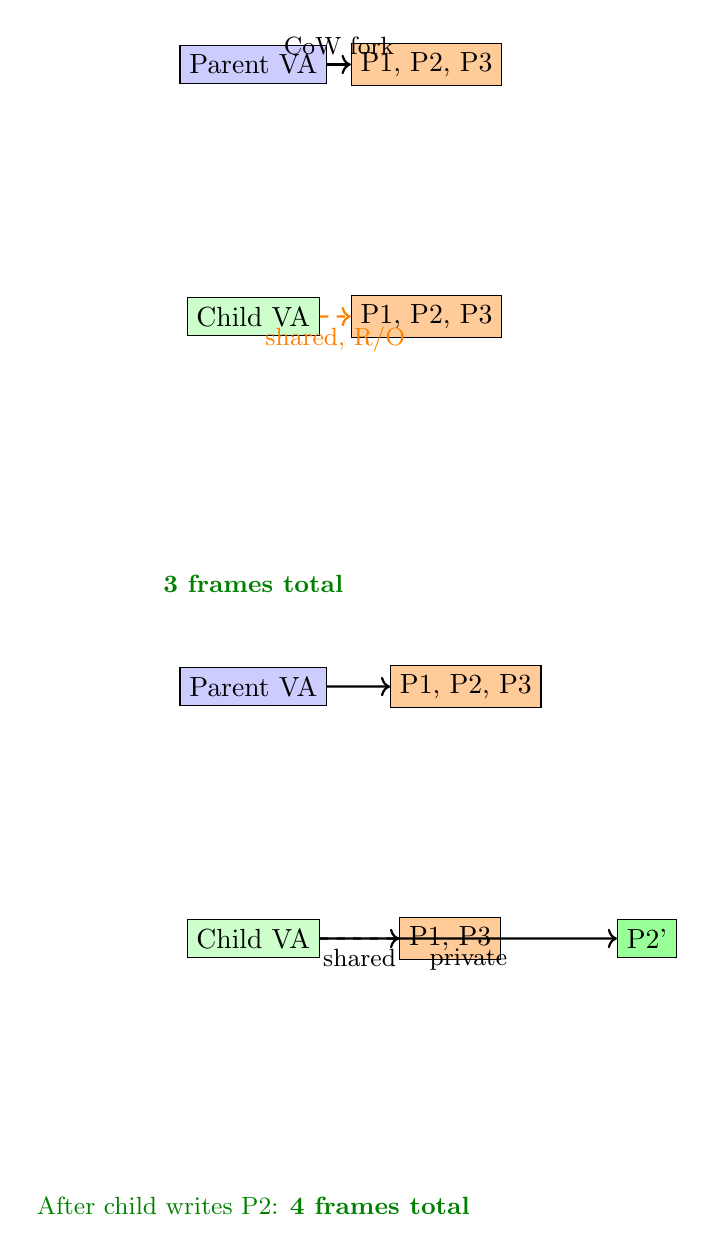
\begin{tikzpicture}[node distance=2.2cm, scale=0.85]
    % Parent side - before
    \node[rectangle, draw, fill=blue!20] (parent_addr) {Parent VA};
    \node[rectangle, draw, fill=orange!40, right of=parent_addr] (parent_frame) {P1, P2, P3};
    \draw[->, thick] (parent_addr) -- (parent_frame) node[midway, above, font=\small] {CoW fork};

    % Child side - before
    \node[rectangle, draw, fill=green!20, below of=parent_addr, yshift=-1cm] (child_addr) {Child VA};
    \node[rectangle, draw, fill=orange!40, right of=child_addr] (child_frame) {P1, P2, P3};
    \draw[->, thick, dashed, color=orange] (child_addr) -- (child_frame) node[midway, below, font=\small] {shared, R/O};

    % Label
    \node[below of=child_addr, yshift=-1.2cm, font=\small, color=green!50!black] {\textbf{3 frames total}};

    % After write
    \node[rectangle, draw, fill=blue!20, below of=child_addr, yshift=-2.5cm] (parent_addr_after) {Parent VA};
    \node[rectangle, draw, fill=orange!40, right of=parent_addr_after, xshift=0.5cm] (parent_frame_after) {P1, P2, P3};
    \draw[->, thick] (parent_addr_after) -- (parent_frame_after);

    \node[rectangle, draw, fill=green!20, below of=parent_addr_after, yshift=-1cm] (child_addr_after) {Child VA};
    \node[rectangle, draw, fill=orange!40, right of=child_addr_after, xshift=0.3cm] (shared_frame_after) {P1, P3};
    \node[rectangle, draw, fill=green!40, right of=shared_frame_after, xshift=0.3cm] (child_only) {P2'};
    \draw[->, thick, dashed] (child_addr_after) -- (shared_frame_after) node[midway, below, font=\small] {shared};
    \draw[->, thick] (child_addr_after) -- (child_only) node[midway, below, font=\small] {private};

    % Label
    \node[below of=child_addr_after, yshift=-1.2cm, font=\small, color=green!50!black] {After child writes P2: \textbf{4 frames total}};
\end{tikzpicture}
\end{center}
\caption{Copy-on-Write fork: initial state shares all pages read-only; on write, a page is duplicated and made private to the writing process.}
\end{figure}

The key advantage of CoW is that fork itself now costs $O(1)$ time and space: the OS only needs to copy page table metadata (the page directory and page tables themselves), not the underlying data. The cost of copying data is deferred and amortized across subsequent writes. If the child exits without writing, no data copy ever occurs. For programs that fork and exec, this is a tremendous win.

\begin{keyidea}
Copy-on-Write trades the synchronous, up-front cost of fork for asynchronous costs distributed across page faults. This is a classic lazy-evaluation pattern: do not pay a cost unless necessary, and defer payment until the need arises.
\end{keyidea}

% ============================================================
\section{Page Tables and Process Isolation: Shared Physical Pages}
% ============================================================

A natural question arises when discussing shared pages: could we reduce the complexity further by sharing the page table itself between processes? If two processes shared a single page directory and the same page tables, they would automatically share all physical pages, and the fork implementation would be trivial.

The answer is a clear \emph{no}, and the reason illuminates a fundamental principle of process isolation. If Process A and Process B share a page directory and page tables, then any modification to those tables by either process immediately affects the other. For example, if Process A allocates a new page and updates the shared page table, Process B would suddenly see that page in its virtual address space. Worse, if Process B writes to that page, the write would be visible to Process A. Isolation between processes would be shattered.

More concretely, consider two processes sharing a page table. Process A and Process B both have virtual address 0x1000 mapping to physical page P. If Process A writes 0xdeadbeef to 0x1000, the write goes to P. If Process B then reads from 0x1000, it sees 0xdeadbeef. The processes are \textbf{not isolated}; they are effectively sharing memory, which violates the memory protection contract.

The solution is clear: \textbf{each process must have its own page directory and page tables}, even if multiple processes share the same underlying physical pages. The page tables are the OS's mechanism for controlling the virtual-to-physical mapping, and these mappings are per-process. Shared physical pages are achieved not by sharing page tables, but by having separate page tables (in separate processes) that point to the same physical frame.

xv6's CoW implementation, as described in Lab 2, does not use CoW page directory or page table allocation. Each process has its own page directory and page tables. Child page tables are copies of parent page tables (with write permissions cleared), not shared references. When the child modifies its virtual address space (e.g., via \texttt{sbrk}), the child's page tables change independently of the parent's.

% ============================================================
\section{Permissions: Logical vs.\ Physical}
% ============================================================

The distinction between \textbf{logical permissions} and \textbf{physical permissions} is central to understanding Copy-on-Write and other advanced paging techniques.

\textbf{Logical permissions} answer the question: ``Is it legal for this process to access this memory?'' These are determined by the OS's policy. In a typical OS, a process has logical write permission to its heap, stack, and data segments, and logical read-only permission to its code segment and memory-mapped files. Logical permissions reflect the intended use of memory and are typically persistent.

\textbf{Physical permissions} answer the question: ``Will the CPU give the MMU a page fault if I try to access this memory?'' These are determined by the bits set in the page table entry, specifically the P (Present), W (Writable), and U (User) bits. Physical permissions are what the hardware enforces.

In a normal scenario, logical and physical permissions align: if a process has logical write permission, the W bit is set, and writes succeed. But CoW breaks this alignment. A page may be \textbf{logically writable} (the process should be able to write to it) but \textbf{physically read-only} (the W bit is clear, so writes trigger a page fault). The OS uses this mismatch as a mechanism to detect write attempts and trigger CoW handling.

To track which pages are CoW (rather than truly read-only), the OS can use the AVL (Available for system use) bits, which are the three least significant bits (bits 9, 10, 11) of the PTE. These bits are ignored by the hardware and reserved for the OS. The OS sets a CoW flag in one of the AVL bits to distinguish a page that is read-only because of CoW from a page that is truly read-only (e.g., a code segment or shared library).

\begin{keytip}
When implementing CoW, always record in the PTE (using AVL bits) whether a page is CoW or truly read-only. A page fault on a write to a truly read-only page should trigger a segmentation fault, not a CoW copy operation.
\end{keytip}

% ============================================================
\section{PTE and PDE Flag Bits Review}
% ============================================================

The page table entry (PTE) and page directory entry (PDE) in xv6 are 32-bit values, with the upper 20 bits forming the physical page number and the lower 12 bits forming flags. Understanding these flags is essential for implementing CoW and other virtual memory features.

\begin{center}
\begin{tabular}{ll}
\toprule
\textbf{Flag} & \textbf{Meaning} \\
\midrule
P (bit 0) & Page is present in physical memory; if clear, page is swapped out or unmapped. \\
W (bit 1) & Page is writable; if clear, write attempts cause a page fault. \\
U (bit 2) & Page is accessible to user mode; if clear, only kernel mode can access. \\
WT (bit 3) & Write-through cache policy. \\
CD (bit 4) & Cache disable. \\
A (bit 5) & Accessed: set by the MMU when the page is read or written. \\
D (bit 6) & Dirty: set by the MMU when the page is written. \\
PS (bit 7) & Page size (0 for 4~KB, 1 for 4~MB pages in 32-bit mode). \\
G (bit 8) & Global: page is not flushed from TLB on CR3 changes. \\
AVL (bits 9--11) & Available for OS use (CoW flags, page type, etc.). \\
\bottomrule
\end{tabular}
\end{center}

For Copy-on-Write implementation, the critical flags are:

\begin{itemize}
    \item \textbf{P (Present):} A page with P~=~0 is not present and will cause a page fault on access. The OS uses this to implement swapping and on-demand allocation.
    \item \textbf{W (Writable):} A page with W~=~0 is not writable; attempting to write will cause a page fault. For CoW, we clear the W bit on shared pages to detect writes.
    \item \textbf{U (User):} A page with U~=~0 is not accessible to user-mode code. This is the boundary between user and kernel memory.
    \item \textbf{AVL (bits 9--11):} The OS can set these bits to mark pages as CoW. Typically, one AVL bit is designated as the CoW flag. When a write fault occurs on a page with the CoW flag set and the W bit clear, the OS knows to copy the page rather than deny access.
\end{itemize}

% ============================================================
\section{Copy-on-Write Example: Detailed Walkthrough}
% ============================================================

Let us walk through a detailed example of Copy-on-Write in action, including the allocation of new page table entries and the handling of reference counts.

\textbf{Initial State:} Consider a system with two processes (Parent and Child) that have just undergone a CoW fork. The parent's virtual address space is laid out as follows:

\begin{itemize}
    \item VA 0x0 $\rightarrow$ PA P1 (Page Table PT1 entry 0), R=1 W=1 (readable, writable).
    \item VA 0x1000 $\rightarrow$ PA P2 (Page Table PT1 entry 1), R=1 W=1.
    \item VA 0x2000 $\rightarrow$ PA P3 (Page Table PT2 entry 0), R=1 W=1.
\end{itemize}

The parent's page directory (PD1) contains:
\begin{itemize}
    \item PDX 0: PD1[0] $\rightarrow$ PT1
    \item PDX 1: PD1[1] $\rightarrow$ PT2
\end{itemize}

After a CoW fork, the child has its own page directory (PD2) and page tables (PT3, PT4). PT3 is a copy of PT1, and PT4 is a copy of PT2. All pages are marked read-only (W bit cleared):

\begin{itemize}
    \item Child VA 0x0 $\rightarrow$ PA P1, R=1 W=0 (shared, read-only).
    \item Child VA 0x1000 $\rightarrow$ PA P2, R=1 W=0 (shared, read-only).
    \item Child VA 0x2000 $\rightarrow$ PA P3, R=1 W=0 (shared, read-only).
\end{itemize}

Both the parent and child also have their read-only bits cleared:
\begin{itemize}
    \item Parent VA 0x0 $\rightarrow$ PA P1, R=1 W=0, CoW flag set (shared, read-only).
    \item Parent VA 0x1000 $\rightarrow$ PA P2, R=1 W=0, CoW flag set.
    \item Parent VA 0x2000 $\rightarrow$ PA P3, R=1 W=0, CoW flag set.
\end{itemize}

Reference counts for the shared pages:
\begin{itemize}
    \item refcount(P1) = 2 (parent and child).
    \item refcount(P2) = 2.
    \item refcount(P3) = 2.
\end{itemize}

\textbf{Scenario: Child writes to P1.} The child executes a store instruction targeting VA 0x0. The MMU performs a page table walk using the child's page directory (PD2) and finds the PTE in PT3. The PTE has P~=~1 (page is present) and W~=~0 (page is not writable). The MMU raises a page fault exception. Control transfers to the OS page fault handler.

The page fault handler examines the faulting address (0x0), the faulting process (child), and the reason for the fault. The handler checks the PTE in PT3:
\begin{itemize}
    \item P bit is set (page is present).
    \item W bit is clear (page is not writable).
    \item CoW flag (an AVL bit) is set, indicating this is a CoW page, not a truly read-only page.
\end{itemize}

The handler decides that this is a CoW fault and proceeds:

\begin{enumerate}
    \item Check the reference count for P1. It is 2, indicating the page is shared.
    \item Allocate a new physical page, P4, from the free page pool.
    \item Copy the contents of P1 into P4 (using the kernel's virtual mappings of both pages).
    \item Update the child's PTE in PT3[0] to point to P4 instead of P1.
    \item Set the W bit in the child's PTE (the child now owns P4 privately).
    \item Clear the CoW flag in the child's PTE (it is no longer CoW).
    \item Decrement refcount(P1) from 2 to 1.
    \item Check if refcount(P1) has dropped to 1. If so, the remaining owner (the parent) has sole access to P1 and should be able to write. However, the parent's PTE still has W~=~0. Ideally, the OS would set the W bit in the parent's PTE and clear the CoW flag, restoring full write access. In practice, xv6 may defer this or skip it for simplicity.
    \item Flush the child's TLB entry for VA 0x0 (using \texttt{invlpg} on x86) to force the MMU to use the new PTE.
    \item Return from the page fault handler and resume the child's execution at the faulting instruction.
\end{enumerate}

After the page fault is handled, the state is:

\textbf{Parent's address space:}
\begin{itemize}
    \item VA 0x0 $\rightarrow$ PA P1, R=1 W=0, CoW flag set (parent still shares with no one, but doesn't know it).
    \item VA 0x1000 $\rightarrow$ PA P2, R=1 W=0, CoW flag set.
    \item VA 0x2000 $\rightarrow$ PA P3, R=1 W=0, CoW flag set.
\end{itemize}

\textbf{Child's address space:}
\begin{itemize}
    \item VA 0x0 $\rightarrow$ PA P4, R=1 W=1 (private, writable).
    \item VA 0x1000 $\rightarrow$ PA P2, R=1 W=0, CoW flag set (still shared with parent).
    \item VA 0x2000 $\rightarrow$ PA P3, R=1 W=0, CoW flag set (still shared with parent).
\end{itemize}

\textbf{Reference counts:}
\begin{itemize}
    \item refcount(P1) = 1 (parent only).
    \item refcount(P2) = 2.
    \item refcount(P3) = 2.
    \item refcount(P4) = 1 (child only).
\end{itemize}

Notice that the parent's write permission was not automatically restored. This is a minor inefficiency: if the parent later tries to write to P1, it will incur another page fault, discover that it is the sole reference, and restore its write bit. In Lab 2, you may opt to restore permissions immediately when refcount drops to 1, or defer the restoration until the next fault.

% ============================================================
\section{TLB Invalidation and Flushes on Copy-on-Write Writes}
% ============================================================

When a page fault occurs and the OS decides to copy a page, an important question arises: how must the TLB be updated? The translation lookaside buffer (TLB) is a small, fast cache of virtual-to-physical address translations maintained by the MMU. If the OS changes a PTE and does not inform the TLB, the MMU may continue to use a stale translation, violating the OS's intent.

In the case of a CoW write fault, the OS allocates a new physical page and updates the faulting process's PTE to point to it. The old translation (faulting virtual address $\rightarrow$ old physical page) is now invalid for this process. The OS must flush this entry from the TLB.

On x86, the \texttt{invlpg} instruction invalidates a single TLB entry by virtual address. The xv6 virtual memory code uses macros like \texttt{lcr3} to flush the entire TLB by reloading the CR3 register (which causes the MMU to discard all non-global TLB entries). For a single CoW fault, invalidating just the one faulting address via \texttt{invlpg} is more efficient than flushing the entire TLB.

\begin{itemize}
    \item \textbf{TLB invalidations} (per-address flushes using \texttt{invlpg}): On a CoW write fault affecting process P, one invalidation is needed for the faulting address in process P's TLB.
    \item \textbf{TLB flushes} (global flushes via CR3 reload): xv6 flushes the entire TLB when switching processes (on context switch), when the kernel page tables are modified, or during certain initialization routines. On a CoW write fault within the same process, no global flush is necessary.
\end{itemize}

\begin{keyidea}
The MMU's TLB is a cache. When the OS modifies a PTE, it must invalidate the corresponding TLB entry, or the MMU will use stale translations. For performance, prefer per-address invalidation (\texttt{invlpg}) over global flushes when possible.
\end{keyidea}

% ============================================================
\section{Building Copy-on-Write: Engineering Decisions and Challenges}
% ============================================================

Implementing Copy-on-Write correctly requires careful engineering decisions and attention to corner cases. The xv6 Lab 2 assignment focuses on CoW fork and write fault handling, but a production implementation must handle many additional scenarios.

\textbf{Reference counting strategy:} The OS must track reference counts per physical page, not per virtual page. A single physical page can be mapped by many virtual address spaces (across different processes), and the OS must know when a page's reference count drops to 1 (sole owner) or to 0 (no owners, can be freed). The reference count can be stored in a global array, indexed by physical page number. When a page is allocated, its refcount is 1. When a new mapping is created (e.g., during CoW fork), the refcount is incremented. When a mapping is removed (e.g., during process exit or CoW copy), the refcount is decremented. When refcount reaches 0, the page is freed and returned to the allocator.

\textbf{Corner case: nested forks.} If a parent forks a child, and the child then forks a grandchild, all three processes may share the same physical pages. The reference count must account for all three. If the parent exits while the child and grandchild still reference a shared page, the refcount decrements from 3 to 2, and the page remains in use. If the child then writes to the page, it must copy and update only its own mappings; the grandchild's page table remains unchanged.

\textbf{Corner case: orphaned pages.} If a parent exits before its child, the child must continue to have access to the shared pages. The OS must not free these pages even though the parent no longer references them. Reference counting handles this correctly: the parent's exit decrements each page's refcount by 1, but pages with grandchildren still have refcount $\geq 1$ and are not freed.

\textbf{Corner case: out-of-memory during copy.} If the system runs low on physical memory and a CoW fault occurs, the OS might not be able to allocate a new page. Some systems defer the copy until memory is available, triggering the process to wait. xv6 simplifies by panicking if \texttt{kalloc} fails, but a production system must handle this gracefully.

\textbf{Resource cleanup on exit:} When a process exits, the OS must decrement the reference count for every physical page the process mapped. This includes pages that were copied during CoW faults (which have refcount 1 for the exiting process) and shared pages (which may have refcount $> 1$). Only pages with refcount 0 are freed. If a process has many pages, this cleanup can be expensive; in xv6, page table walking and cleanup happen synchronously in the \texttt{freevm} function.

\textbf{CoW flag management:} The OS must be able to distinguish CoW pages (logically writable but physically read-only) from truly read-only pages (logically read-only, e.g., code segments). Using an AVL bit to mark CoW pages is essential. When a page is copied and becomes private, the CoW flag is cleared. When two pages are newly shared (e.g., after fork), the CoW flag is set in both page tables.

\textbf{Restore write permissions:} When a page's reference count drops to 1 (sole owner), the OS can restore the W bit in the sole owner's PTE, eliminating the need for future faults on that page. However, this requires the OS to find the PTE and update it, which may require scanning page tables or maintaining a reverse mapping data structure. xv6's simple implementation may skip this optimization.

% ============================================================
\section{Copy-on-Write Page Fault Handling Flow}
% ============================================================

The following diagram illustrates the sequence of events when a CoW write fault occurs and is handled by the OS.

\begin{figure}[h]
\begin{center}
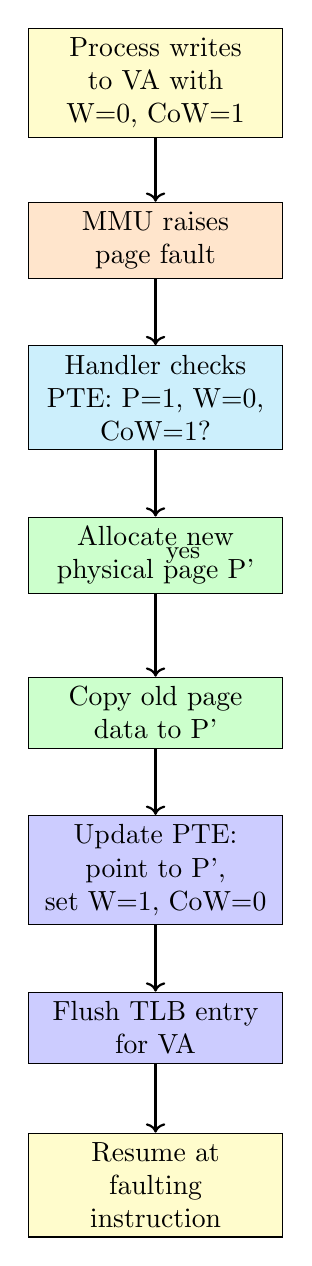
\begin{tikzpicture}[node distance=2cm, scale=0.85]
    % Start
    \node[rectangle, draw, fill=yellow!20, text width=3cm, align=center] (start) {Process writes\\to VA with\\W=0, CoW=1};

    % Page fault
    \node[rectangle, draw, fill=orange!20, below of=start, text width=3cm, align=center] (fault) {MMU raises\\page fault};
    \draw[->, thick] (start) -- (fault);

    % Handler checks
    \node[rectangle, draw, fill=cyan!20, below of=fault, text width=3cm, align=center] (check) {Handler checks\\PTE: P=1, W=0,\\CoW=1?};
    \draw[->, thick] (fault) -- (check);

    % Allocate
    \node[rectangle, draw, fill=green!20, below of=check, text width=3cm, align=center] (alloc) {Allocate new\\physical page P'};
    \draw[->, thick] (check) -- (alloc) node[right, font=\small] {yes};

    % Copy
    \node[rectangle, draw, fill=green!20, below of=alloc, text width=3cm, align=center] (copy) {Copy old page\\data to P'};
    \draw[->, thick] (alloc) -- (copy);

    % Update PTE
    \node[rectangle, draw, fill=blue!20, below of=copy, text width=3cm, align=center] (update) {Update PTE:\\point to P',\\set W=1, CoW=0};
    \draw[->, thick] (copy) -- (update);

    % Flush TLB
    \node[rectangle, draw, fill=blue!20, below of=update, text width=3cm, align=center] (tlb) {Flush TLB entry\\for VA};
    \draw[->, thick] (update) -- (tlb);

    % Resume
    \node[rectangle, draw, fill=yellow!20, below of=tlb, text width=3cm, align=center] (resume) {Resume at\\faulting\\instruction};
    \draw[->, thick] (tlb) -- (resume);
\end{tikzpicture}
\end{center}
\caption{Copy-on-Write page fault handling flow. The OS detects a write to a shared page and copies it, making it private to the writing process.}
\end{figure}

The sequence is:
\begin{enumerate}
    \item A process executes a store instruction targeting a virtual address whose PTE has W~=~0 (not writable).
    \item The MMU cannot satisfy the write and raises a page fault exception, saving the faulting address and other context.
    \item The OS page fault handler is invoked. It inspects the PTE corresponding to the faulting address.
    \item If the PTE has P~=~1 (present), W~=~0 (not writable), and the CoW flag is set, the handler infers that this is a CoW fault.
    \item The handler allocates a new physical page and copies the contents of the old page into it.
    \item The handler updates the faulting process's PTE to point to the new page, sets the W bit, and clears the CoW flag.
    \item The handler invalidates the TLB entry for the faulting address (using \texttt{invlpg} on x86).
    \item The handler returns from the exception, and the process resumes execution at the faulting instruction. This time, the instruction succeeds because the page is now writable.
\end{enumerate}

% ============================================================
\section{Summary}
% ============================================================

\begin{itemize}
    \item \textbf{Software page walk}: The \texttt{walkpgdir} function performs a two-level page table walk, extracting the directory and table indices from the virtual address and returning a pointer to the corresponding PTE.

    \item \textbf{xv6 limitations}: xv6 does not support many-to-one virtual-to-physical mappings or per-page reference counting, which prevents efficient Copy-on-Write and shared memory features available in production OSes.

    \item \textbf{Level of indirection}: Paging allows the OS to observe and intercept memory accesses by setting permissions more strictly than logically necessary, deferring work until a fault occurs.

    \item \textbf{Fork complexity}: Standard fork copies all address space, costing $O(n)$ time and space. Copy-on-Write fork costs $O(1)$ at fork time and $O(1)$ amortized per write, deferring copying until necessary.

    \item \textbf{Shared pages and isolation}: Multiple processes can map the same physical page if each has its own page directory and page table. The page table entries control each process's permissions independently.

    \item \textbf{Logical vs.\ physical permissions}: A page can be logically writable but physically read-only (W~=~0) to trigger page faults on writes, enabling CoW and other OS tricks.

    \item \textbf{PTE flags}: The P (Present), W (Writable), U (User), and AVL (Available) bits in PTEs are essential for implementing CoW. The AVL bits mark pages as CoW to distinguish them from truly read-only pages.

    \item \textbf{Reference counting}: Each physical page must have a reference count tracking how many processes map it. When refcount reaches 1, the sole owner can be granted write permission. When refcount reaches 0, the page is freed.

    \item \textbf{CoW write fault}: A write to a physically read-only CoW page triggers a page fault. The handler allocates a new page, copies the shared page into it, updates the PTE, and invalidates the TLB entry.

    \item \textbf{TLB invalidation}: After modifying a PTE, the OS must invalidate the corresponding TLB entry using \texttt{invlpg} (per-address) or CR3 reload (global flush). For CoW, per-address invalidation is more efficient.

    \item \textbf{Engineering challenges}: Nested forks, orphaned pages, out-of-memory handling, resource cleanup, and CoW flag management all complicate a production CoW implementation.
\end{itemize}

% ============================================================
\section{References}
% ============================================================

\begin{itemize}
    \item Intel Corporation. ``Intel 64 and IA-32 Architectures Software Developer's Manual.'' Volume 3: System Programming Guide. Retrieved from \url{https://www.intel.com/content/www/us/en/architecture-and-technology/64-ia-32-architectures-software-developer-manual-325384.html}.

    \item University of Washington, CSE 451 Operating Systems. ``Copy-on-Write'' and ``Virtual Memory.'' Course materials. Retrieved from \url{https://courses.cs.washington.edu/courses/cse451/}.

    \item Silberschatz, A., Galvin, P.~B., and Gagne, G. ``Operating System Concepts,'' 10th ed. Wiley, 2018.

    \item Massachusetts Institute of Technology, Course 6.828 Operating System Engineering. ``xv6 Code and Labs.'' Retrieved from \url{https://pdos.csail.mit.edu/6.828/2023/}.

    \item Frans Kaashoek and Robert~T.\ Morris. ``xv6: A Simple Unix-like Teaching Operating System.'' Retrieved from \url{https://github.com/mit-pdos/xv6-public}.
\end{itemize}

% ============================================================
\section*{Personal Notes}
% ============================================================
% Add your own notes below this line

\end{document}
